\documentclass[11pt]{article}
\usepackage[margin=1in]{geometry}
\usepackage{amsmath,booktabs,graphicx,hyperref}
\hypersetup{hidelinks}
\title{Ten-Feature Additive SAE Interventions:\\ Measurable Image Changes and Limits of Semantic Interpretation}
\author{Exploratory research summary}
\date{November 16, 2026}
\begin{document}\maketitle
\begin{abstract}
We summarize existing single-coordinate interventions for ten features of a face-fine-tuned mid.0 sparse autoencoder (SAE). No new diffusion images are generated. The data comprise 4,200 edited images over twelve prompt groups, five paired seeds, and seven additive strengths. We distinguish nonzero image changes from reliable semantic control. Weak or inconsistent responses do not identify an intrinsic racial cause, nor prove that the tested coordinates have no effect.
\end{abstract}
\section{Question and experimental scope}
The original question is whether apparent demographic selectivity arises from sparse activation or from context-dependent intervention behavior. The SAE checkpoint is \path{layers/runs/mid0_sae_face_001/sae}, with SHA-256:
\begin{quote}\scriptsize\texttt{cbb3a0a2d0c43c822c7ba97a494de38ae56ea25401a8d31484ffa32e7cc329a6}\end{quote}
 The diffusion generator is the same frozen SDXL Turbo model; the layer is \path{unet.mid_block.attentions.0}. Sampling is single-step. No weights are trained or updated.
\section{Intervention definitions}
For selected feature $i$, decoder direction $w_i$, and original block output $h$, the residual-preserving intervention is
\[
 h'_{xy}=h_{xy}+\Delta z_i(x,y)w_i,\qquad
 \Delta z_i^{\mathrm{mult}}=(\alpha-1)z_i,\quad
 \Delta z_i^{\mathrm{add}}=\beta.
\]
Multiplication cannot change a coordinate that is zero. Addition can introduce that coordinate at all spatial positions. Neither intervention guarantees a monotonic semantic effect. Uniform addition can exceed the encoder's natural Top-$K$ support and does not reproduce a naturally localized activation pattern. The experiment records actual block-output perturbation norms after precision casting.
\section{Existing-image measurements}
Pixel MAE is the mean absolute RGB difference from the paired no-intervention image on the $0$--$255$ scale. SSIM is a structural-similarity proxy; neither is a validated beard, demographic, identity, or perceptual-quality measurement.
Across all 4,200 edits, 0 images are exactly pixel-identical to baseline. Pixel MAE ranges from 0.2824 to 23.1654; SSIM ranges from 0.6528 to 0.9975. Thus the edits are not generally literal no-ops.
\begin{table}[ht]\centering\small
\begin{tabular}{rrrrrr}\toprule
Feature & Inactive & Matched-small & Matched-moderate & Add $50$ & Exact no-ops\\
 & contexts & MAE & MAE & MAE & \\\midrule
4228 & 34/60 & 0.701 & 0.917 & 7.135 & 0/420  \\
4554 & 16/60 & 0.580 & 1.054 & 8.022 & 0/420  \\
1650 & 34/60 & 0.585 & 0.653 & 6.866 & 0/420  \\
4586 & 27/60 & 0.546 & 0.678 & 5.693 & 0/420  \\
5094 & 33/60 & 0.578 & 0.868 & 6.468 & 0/420  \\
2023 & 19/60 & 0.588 & 1.129 & 5.958 & 0/420  \\
1074 & 31/60 & 0.531 & 0.746 & 5.743 & 0/420  \\
4338 & 5/60 & 1.379 & 1.829 & 9.663 & 0/420  \\
2361 & 17/60 & 0.786 & 1.143 & 11.067 & 0/420  \\
4399 & 10/60 & 0.577 & 0.890 & 6.785 & 0/420  \\
\bottomrule\end{tabular}
\caption{All prompt groups and five paired seeds. Matched perturbation targets differ across features; these columns are not a dose-controlled ranking of features. Inactive counts refer to sixty original prompt/seed contexts.}
\end{table}
\section{Interpretation and causal limits}
The appropriate conclusion is that the tested coordinates produce measurable image changes, while reliable, monotonic semantic control has not been established by these measurements. We do not summarize the result as ``additive features do nothing.'' Feature 4228 is a demographic-associated candidate, not a proven beard-control feature.

In a conditional generator $I=G(c,\epsilon;h)$, changing one coordinate while retaining prompt conditioning $c$ and the surrounding representation does not isolate the mechanism responsible for the original appearance. Prompt wording, other coordinates, spatial structure, feature interactions, intervention timing, and measurement sensitivity remain alternative explanations. A weak response to the tested edit therefore does not imply that ``race itself'' causes the outcome. Prompt race categories are conditioning text, not experimentally isolated biological variables.

Formal evidence of negligible semantic effects would require a defined semantic outcome, a justified equivalence margin, and adequate uncertainty assessment. Pixel similarity or an unchanged classifier label alone is insufficient. This analysis contains no validated all-feature beard or attribute-coverage measurement.
\section{Uncertainty and preservation}
The independent resampling units are five paired recipient seeds, not 4,200 independent images. Reported CSV confidence intervals resample whole seed clusters, retaining all twelve prompt groups. Active and inactive contexts are observational strata whose prompt composition differs. These comparisons are exploratory and cannot establish causal demographic specificity.

All original images and activation archives are retained. The gallery uses existing seed-30 images for all ten features and twelve prompt groups; selection is fixed rather than based on visually striking outcomes. Multiplicative and additive gallery columns are different parameterizations, not magnitude-matched comparisons. Source paths, hashes, per-image measurements and complete confidence intervals accompany this report.
\begin{figure}[ht]\centering
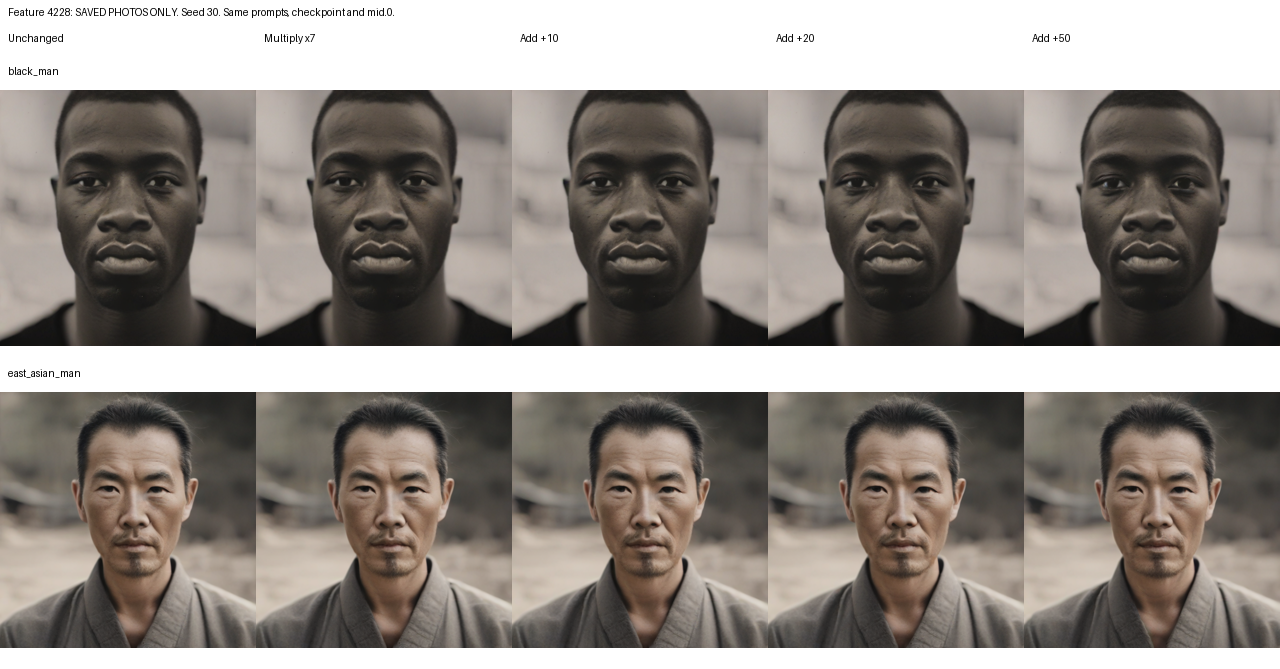
\includegraphics[width=\linewidth]{gallery/feature_4228_two_contexts.png}
\caption{Saved feature-4228 photos. Columns: unchanged, multiplication by7, addition of10,20,50. Rows: Black-man and East-Asian-man prompt contexts, seed30. These are viewing derivatives of existing originals, not new generations or evidence of a semantic null.}
\end{figure}
\end{document}
